% ============================================================
% 3  The lattice model, its order parameter, true LRO
% ============================================================
\begin{frame}[t]
\ft{A chain of spinful fermions}
\begin{columns}[T]
\begin{column}{0.50\textwidth}
\centering
\vspace{0.5cm}
\begin{tikzpicture}[x=0.74cm,y=1.15cm,
  up/.style={-{Stealth[length=3pt]},thick,cLL!80!black},
  dn/.style={-{Stealth[length=3pt]},thick,cFM}]
 \draw[mygray,thick] (-0.3,0)--(6.3,0);
 \foreach \i in {0,...,6} \fill[mygray] (\i,0) circle (0.07);
 % hopping
 \draw[up] (0,0.08)--(0,0.42);
 \draw[-{Stealth[length=3pt]},thin] (0.1,0.5) to[bend left=50] node[above,font=\scriptsize]{$t$} (0.9,0.5);
 % on-site U
 \draw[up] (1.93,0.08)--(1.93,0.42); \draw[dn] (2.07,0.42)--(2.07,0.08);
 \node[font=\scriptsize] at (2,0.68) {$U$};
 % V++
 \draw[up] (3,0.08)--(3,0.42); \draw[up] (4,0.08)--(4,0.42);
 \draw[cQCP,densely dashed,thick] (3.1,0.25)--(3.9,0.25);
 \node[font=\scriptsize,cQCP] at (3.5,0.68) {$V_{++}$};
 % V+-
 \draw[up] (5,0.08)--(5,0.42); \draw[dn] (6,0.42)--(6,0.08);
 \draw[densely dashed,thick] (5.1,0.25)--(5.9,0.25);
 \node[font=\scriptsize] at (5.5,0.68) {$V_{+-}$};
\end{tikzpicture}\par
\vspace{0.4cm}
{\small\setlength{\tabcolsep}{6pt}\renewcommand{\arraystretch}{1.35}
\begin{tabular}{@{}l l@{}}
 $t=1$ & hopping\\
 $U=0.1$ & on-site repulsion\\
 $V_{+-}=0.8$ & neighbours, $\uparrow\downarrow$\\
 \rowcolor{cQCP!15} $\Delta V=V_{++}-V_{+-}$ & \textbf{tuning knob}\\
\end{tabular}\par}
\vspace{0.3cm}
{\scriptsize $\tfrac14$ filling per spin, $k_F=\pi/4$;\ \ symmetry U(1)$\rtimes\mathbb Z_2$\par}
\vspace{0.1cm}
{\tiny\color{citegray} K.~Yang, PRL 93, 066401 (2004)\par}
\end{column}
\begin{column}{0.48\textwidth}
\centering
\vspace{0.35cm}
\onslide<2->{%
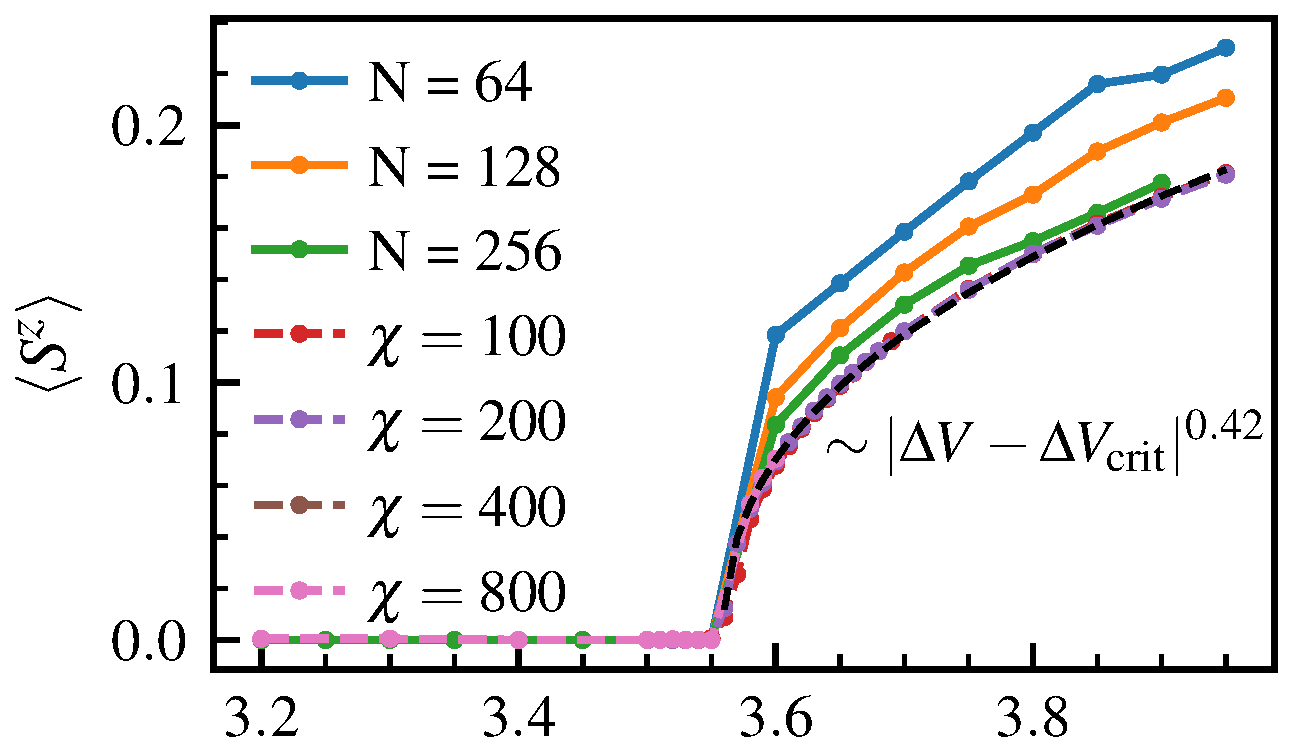
\includegraphics[width=\linewidth]{figures/paper_figS6_magnetization.png}\par
\vspace{0.1cm}
{\footnotesize $\langle S^z\rangle$ sets in continuously at \colorbox{cQCP!15}{\mystrut $\Delta V_\text{crit}\approx3.55$}\par}
{\scriptsize finite DMRG ($N$) and iDMRG ($\chi$)\par}
\vspace{0.25cm}
{\footnotesize \colorbox{citron!40}{\mystrut $K_s\to\infty$}: spin sector $=$ Lifshitz theory\par}}
\end{column}
\end{columns}
\end{frame}
% Notes: This is my part: a concrete lattice model where K_s really diverges. Electrons with spin on a chain, quarter filling per spin.
% Notes: Hopping t, tiny on-site U, and nearest-neighbour density interactions that depend on the spins: same spin V++, opposite spin V+-. The knob is the difference Delta V.
% Notes: K. Yang showed the spin sector of such a model is exactly the compact Lifshitz theory near the ferromagnetic transition.
% Notes: Step 2: DMRG (finite chains N=64,128,256, and infinite iDMRG). The magnetization switches on continuously at Delta V_crit ~ 3.55: second-order transition, ~|dV-dVc|^0.42. Phase separation on the FM side, as Nahum predicted.


\begin{frame}[t]
\ft{Which operator orders?}\par
\vspace{0.5cm}
\begin{columns}[c]
\begin{column}{0.46\textwidth}
\centering
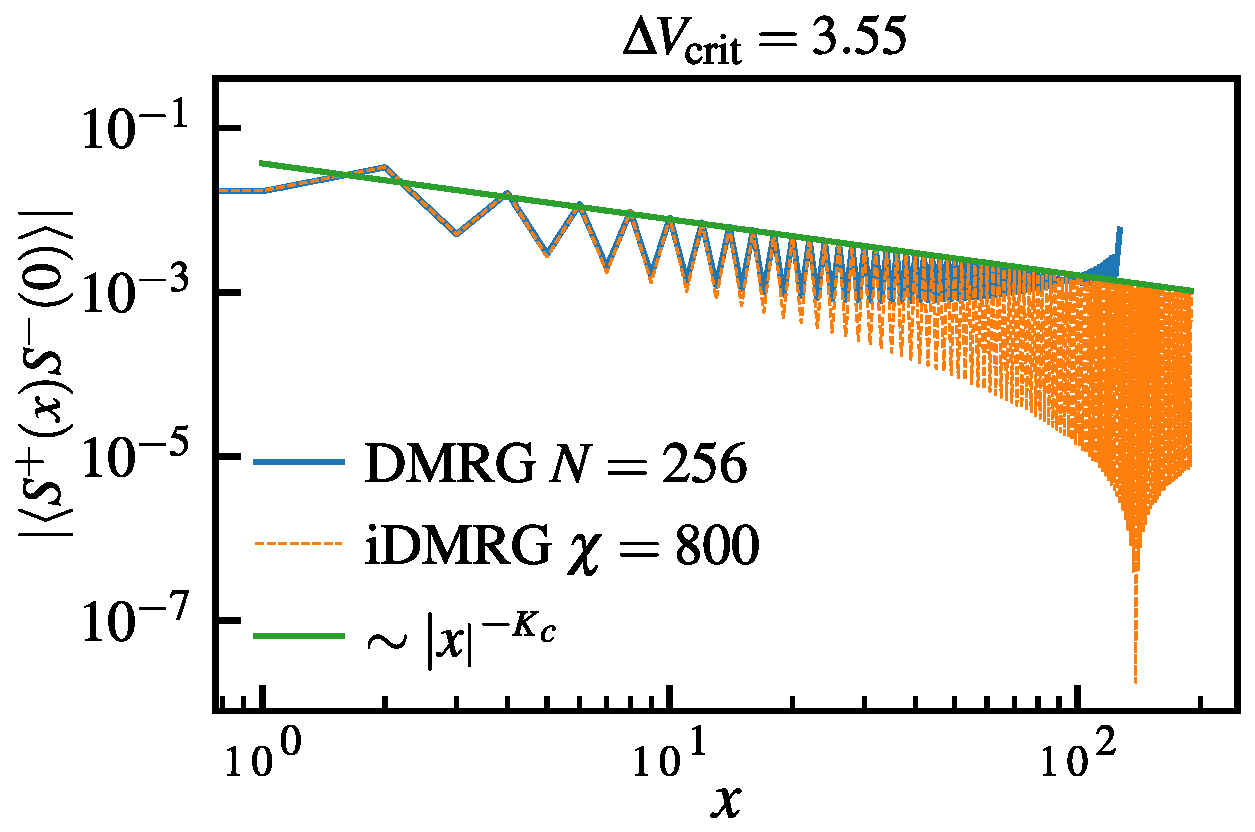
\includegraphics[width=\linewidth]{figures/paper_fig2_splus.png}\par
\vspace{0.05cm}
{\scriptsize $\langle S^+_xS^-_0\rangle$ at the QCP: still a power law\par}
\end{column}
\begin{column}{0.52\textwidth}
{\small
\colorbox{mygraylight}{\mystrut Spin flip}\\[5pt]
$S^+_i\sim e^{-i\sqrt{2\pi}\theta_s}\big[\cos\sqrt{2\pi}\phi_c+\dots\big]$\\[2pt]
{\footnotesize carries the \colorbox{pumpkin!50}{\mystrut charge} Luttinger liquid along\par}
\vspace{0.6cm}
\onslide<2->{%
\colorbox{citron!40}{\mystrut Spin nematic}\\[5pt]
$\mathcal O_i=S^+_iS^+_{i+1}\sim e^{-i\sqrt{8\pi}\theta_s}=e^{-2i\theta}$\\[2pt]
{\footnotesize pure spin sector; spin 2, breaks U(1)$\to\mathbb Z_2$\par}}}
\end{column}
\end{columns}
\onslide<2->{\tk{Pair two spin flips to leave the charge behind}}
\end{frame}
% Notes: On the lattice we must pick an operator. In a pure spin chain S^+ would be the order parameter. In our itinerant chain, bosonization shows S^+ also contains a charge-sector vertex (phi_c), and the charge sector stays a Luttinger liquid. So S^+ only has quasi-long-range order even at the QCP (figure: power law with 2k_F oscillations).
% Notes: Step 2: the product of two neighbouring spin flips: the charge parts cancel (Klein-factor bookkeeping in the supplement). It is a pure theta_s vertex, e^{-2i theta}: a spin-2 "nematic" operator, breaks U(1) down to Z2.


\begin{frame}[t]
\ft{True long-range order at the critical point}\par
\vspace{0.45cm}
\begin{columns}[c]
\begin{column}{0.60\textwidth}
\centering
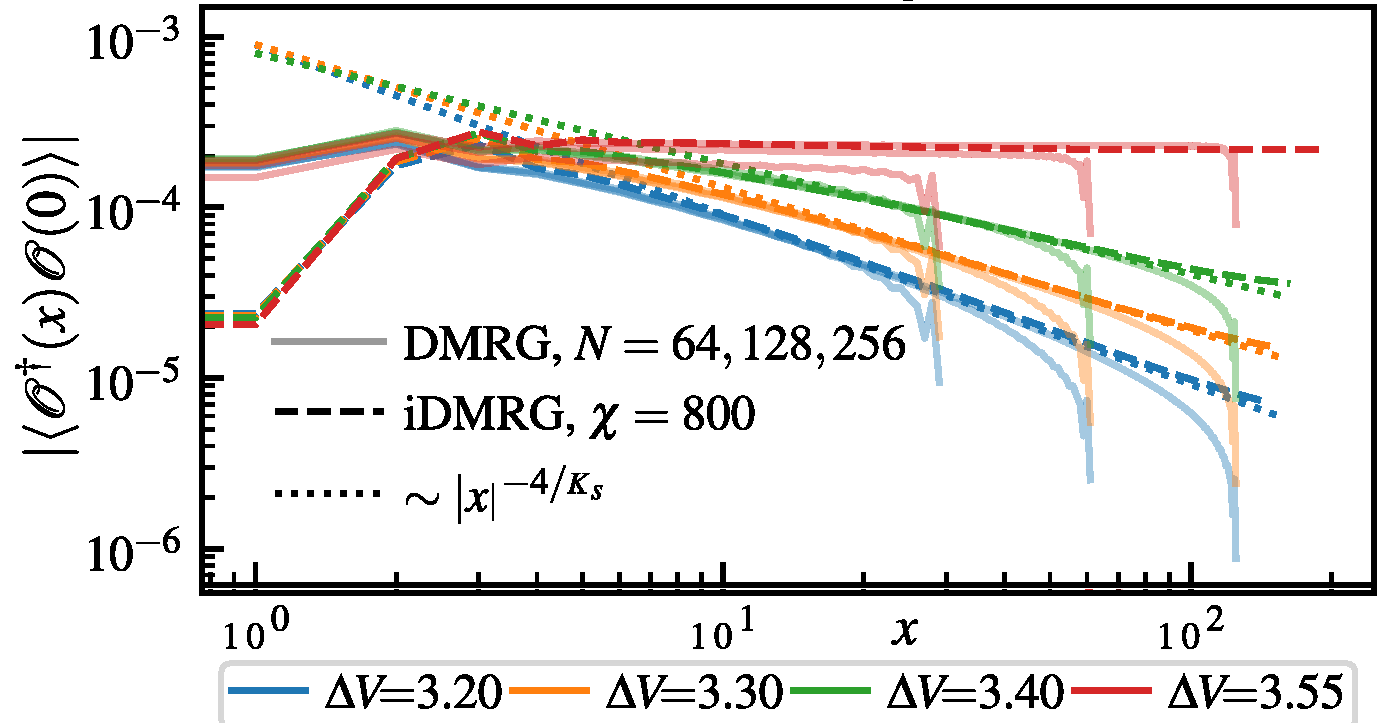
\includegraphics[width=\linewidth]{figures/paper_fig1_nematic.png}\par
\vspace{0.05cm}
{\tiny\color{citegray} Andriyakhina, Shankar, Senthil, Shi, arXiv:2609.38581 (2026)\par}
\end{column}
\begin{column}{0.38\textwidth}
\colorbox{cLL!20}{\mystrut Luttinger liquid}\\[3pt]
\hspace*{0.3cm}$\langle\mathcal O^\dagger_x\mathcal O_0\rangle\sim|x|^{-4/K_s}$\\[2pt]
\hspace*{0.3cm}{\footnotesize slower as $K_s$ grows\par}
\vspace{0.4cm}
\onslide<2->{\colorbox{cQCP!15}{\mystrut Critical point}\\[3pt]
\hspace*{0.3cm}$\langle\mathcal O^\dagger_x\mathcal O_0\rangle\to$ const\par}
\vspace{0.4cm}
\onslide<3->{\colorbox{citron!40}{\mystrut Nematic order only}\\[3pt]
\hspace*{0.3cm}$\langle S^z\rangle=\langle S^\pm\rangle=0$\par}
\end{column}
\end{columns}
\onslide<2->{\tk{An ordered critical point in one dimension}}
\end{frame}
% Notes: Nematic correlator vs distance, log-log. Blue/orange/green: Luttinger liquid at increasing Delta V; dotted lines are |x|^{-4/K_s} with K_s from the LL fits: the decay gets slower as we approach the QCP.
% Notes: Step 2: red, at Delta V_crit: the correlator saturates to a constant, both in finite chains (faded, up to boundary effects) and in iDMRG (dashed). True long-range order.
% Notes: Step 3: no magnetization, no ordinary transverse order (S+S- is only QLRO), but spin-nematic LRO. The naive "K_s -> infinity" picture gives the right answer here, but the critical point is not a Luttinger liquid: next slides.
